\section{Background and Existing Works}
\label{Sec:Background}

\begin{figure*}[h]
\centering
\subfloat[Naive Burst-Buffer Aware Scheduler, e.g. SLURM] {
        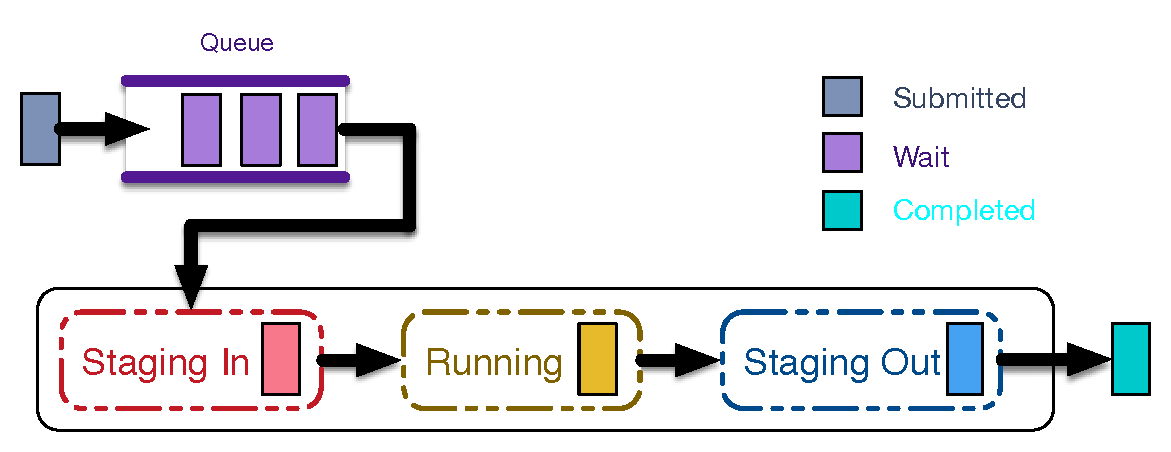
\includegraphics[width=3.1in]{SlurmQueue}
        \label{Fig:SlurmQueue}
}
\subfloat[Job Movement in Cerberus's Multiple Queues] {
        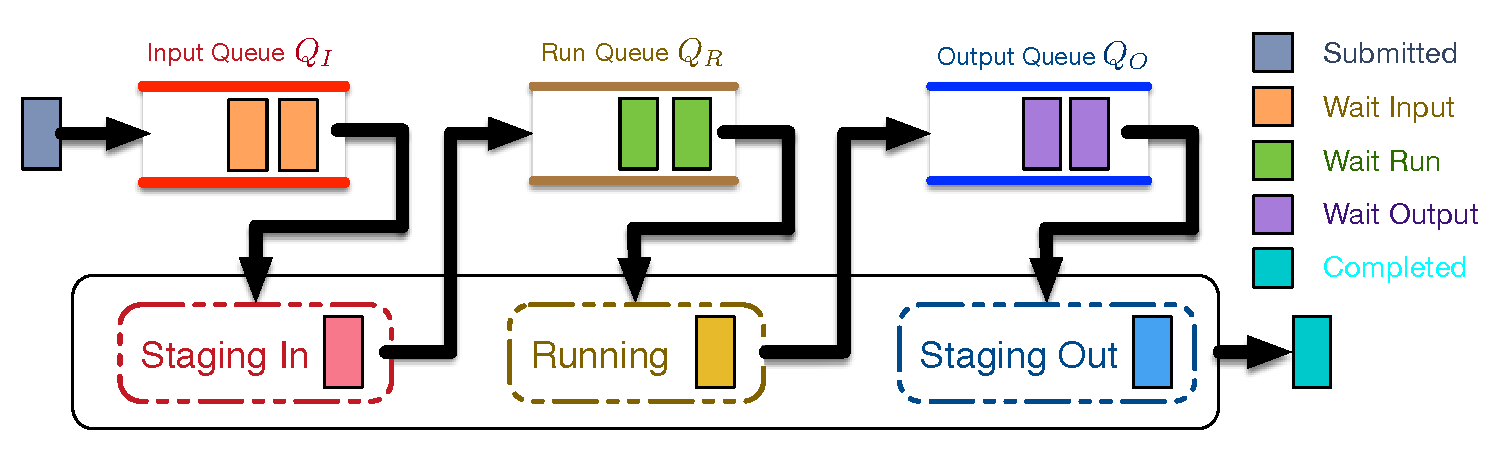
\includegraphics[width=3.7in]{CerberusQueues}
        \label{Fig:CerberusQueues}
}
\caption{Architecture Comparison: Single-Queue Adopted by Existing Batch Scheduler v.s. Multiple-Queue Used by Cerberus}
\label{Fig:CompareSlurmCerberus}
\end{figure*}

%1. The appear of burst buffer
Burst buffer enabled I/O architecture can help alleviate
the ever-increasing I/O pressure on HPC systems.
It debuts as a rescue by utilizing various new storage technologies,
such as non-volatile random-access memory (NVRAM) and solid state drive (SSD).
In practice, burst buffer suits up with DataWarp I/O accelerator\cite{DataWarp}.
Figure \ref{Fig:BBArchitecture} illustrates one burst-buffer-enabled architecture,
adopted by the Trinity System\cite{TrinitySystem}.
%The volume of data read/write may affect the architecture model of burst buffer.
In Trinity, the burst buffer node is composed of one I/O node and 2 PCIe SSD cards,
connected via 16 PCIe 3.0 interfaces.
Alternatively, many researchers have proposed to distribute burst buffer 
on multiple layers of the memory hierarchy\cite{Romanus:CORR:15}.
For example, they may be deployed on the local compute nodes, the board in the cabinet or the I/O nodes.
Burst buffer may also be utilized as the intermediate storage systems.

%2. Use cases of burst buffer
Regardless of the specific deployment, burst buffer nodes essentially augment
the I/O stack with an intermediate productive offloading layer, 
which can benefit jobs in multiple ways.
As discussed in some preliminary surveys\cite{apex-workflow} ,
jobs' latest checkpoints can be pre-staged
before the previous job terminates;
jobs can burst checkpoint to burst buffer
with extremely high speed (4.4-17.8 TB/s on Trinity);
upon termination, jobs are also able to drain off output data
asynchronously to the external parallel file system (PFS).
The bursty I/O operations can thus be aggregated and absorbed into the burst buffer,
which shifts the computation that follows the I/O bursts to an earlier moment,
while burst buffer nodes take charge of moving potentially TB-level volumes of data.
There are more use cases for burst buffer nodes.
Among them, \textit{data cache} is equally important to enhance the responsiveness
of applications by improving the perceived I/O bandwidth\cite{TrinitySystem}.
Shared object library or read-only configuration files are cached into burst buffer;
a list of input files specific to a group of compute nodes allocated to
a particular job is loaded into burst buffer prior to the execution.
Economical solid-state disks as a tier of burst buffer could also be used as
out-of-core complement of insufficient main memory\cite{Romanus:CORR:15},
or working place for data analysis (reductions, feature extraction compression etc.)
and visualization\cite{TrinitySystem}.

%3. Existing works SLURM as example
Given the critical role of burst buffer in future HPC systems,
users are encouraged to explicitly request this new resource for performance enhancement\cite{apex-workflow}.
Inspired by this requirement, it is necessary to holistically manage
the allocation of these precious I/O resources,
which naturally falls into the responsibilities of the batch scheduler.
Existing batch schedulers \cite{Moab, Cobalt, SlurmBBGuide, PBSonCRAY} have already claimed to
be aware of burst buffer, but in fact only deals with it in a naive way.

Figure~\ref{Fig:SlurmQueue} depicts the way existing burst-buffer-aware scheduler manages burst buffer.
For example, SLRUM developed a module that allocates burst buffer resources to the submitted user jobs.
The module extra considers if jobs' burst buffer requirements are met when making scheduling decision.
With the pre-allocated burst buffer,
the I/O performance of user jobs indeed can be improved\cite{SlurmBBGuide}.
PBS supports burst buffer aware scheduling in similar way as SLURM:
jobs are only dispatched when both required burst buffer and computing resource are ready\cite{PBSonCRAY}.

%4. Problem of existing schedulers
However, there are three problems in such single-queueing framework.
First, even though job's lifetime is conceptionally divided into 3 phases
(e.g. staging in, running and staging out) by the existing batch schedulers like SLURM,
they are in fact just the running phase because scheduler cannot do anything once a job is kicked off.
Secondly, a dispatched job will keep taking up its computing nodes and burst buffer nodes during entire execution.
One may argue that there are cases that a job only need burst buffer to do I/O operations,
and there are cases that job can release computing nodes as soon as computation results are buffered
in burst buffer.
Finally, burst buffer and computing nodes are allocated altogether
in the straightforward first-come, first-served manner, without doing any optimization.
In conclusion, the static burst-buffer-aware scheduling framework in Figure~\ref{Fig:SlurmQueue}
is far from fully exploiting the utilization of burst buffer.

%5. Brief intro about our works
This paper aims to bridge the two isolated fields of HPC architecture:
the novel burst buffer equipped with HPC I/O subsystem and the
traditional batch job queueing subsystem.
The bridge builds upon a three-phase job model motivated by critical use cases of burst buffer.
In three-phase job model, users are encouraged to provide the burst buffer demand on submission
and the execution of job is modeled into stage-in, running and stage-out phases.
The user jobs will acquire different resources before entering each phase.
This three-phase job model enables our burst-buffer-aware scheduler, Cerberus,
to adopt the scheduling framework illustrated in Figure~\ref{Fig:CerberusQueues}.

Comparing with the existing batch scheduler like SLRUM and PBS,
our approach have the following advantages.The most difference is that there are three queues in Cerberus.
In three phase model, job demands different kind of resources at each phase.
Cerberus can deal with different resource demand by holding jobs in particular phase in designated queue.
Besides, the finer granularity introduced by more queues can further exploit
both the computing nodes and burst buffer nodes.
When finishing each phases, job will release its acquired resources, making it possible
to be allocated to other jobs promptly.
For example, when the golden job, in Figure~\ref{Fig:CerberusQueues}, finishes running, it will release the burst buffer it used to
do checkpointing, which can be immediately available to jobs in any phases.
We also integrate queues in Cerberus with different optimization algorithms for the
objective of maximizing the resource utilization and the system throughput.

In the following sections, we demonstrate that when burst buffer is intelligently allocated
by our novel batch scheduler, the benefit is far beyond the higher hardware transfer bandwidth.
The job execution is expedited by having their bursty I/O requests absorbed by burst buffer.
The job waiting time is reduced via the contracted input/output stage in the scheduling pipeline.
To our best knowledge, this is the first attempt to holistically research job scheduling
on the new burst-buffer-enabled HPC systems.

